\chapter{Classi astratte}
\section{Interfacce sviluppate}
\begin{enumerate}
	\item Audio.h;
	\item Input.h;
	\item Light.h;
	\item LightPwm.h.
\end{enumerate}

\subsection{Audio.h}
Questa classe è l'astrazione della gestione di eventi sonori, in cui ogni suono da emettere dovrebbe avere un numero univoco assegnato. All'interno del sistema viene implementata dalle classi Buzzer.
\subsubsection{Metodi}
\begin{itemize}
	\item \texttt{public virtual void playSound(int) = 0}
\end{itemize}
\begin{figure}[!ht]
	\centering
	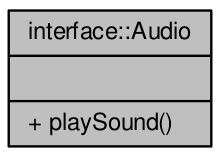
\includegraphics[scale=.35]{img/UML/CollaborationDiagram/interface/interface::Audio.png}
	\caption{Collaboration Diagram - interface::Audio}
\end{figure}
\begin{figure}[!ht]
	\centering
	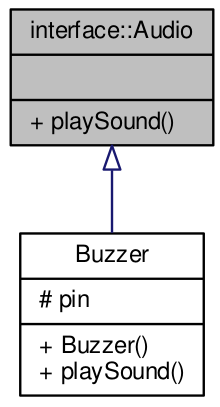
\includegraphics[scale=.35]{img/UML/InheritanceDiagram/interface/interface::Audio.png}
	\caption{Inheritance Diagram - interface::Audio}
\end{figure}

\newpage
\subsection{Input.h}
Questa classe è l'interfaccia da implementare per gestire gli eventi di input da parte dei vari device, che nel progetto sono il sonar e il button.
\subsubsection{Metodi}
\begin{itemize}
	\item 	\begin{verbatim}
	virtual bool readBool() {
	   	return false;
	};
	\end{verbatim}
	\item 	\begin{verbatim}
	virtual int readDistance() {
	   	return 0;
	};
	\end{verbatim}
\end{itemize}
\begin{figure}[!ht]
	\centering
	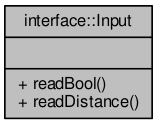
\includegraphics[scale=.5]{img/UML/CollaborationDiagram/interface/interface::Input.png}
	\caption{Collaboration Diagram - interface::Input}
\end{figure}
\begin{figure}[!ht]
	\centering
	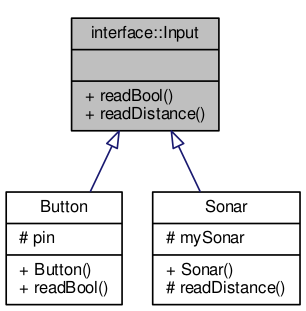
\includegraphics[scale=.5]{img/UML/InheritanceDiagram/interface/interface::Input.png}
	\caption{Inheritance Diagram - interface::Input}
\end{figure}

\newpage
\subsection{Light.h}
Questa interfaccia rappresenta la gestione dei LED attraverso la loro accensione/spegnimento al fine di dare un feedback visivo al giocatore.
\subsubsection{Metodi}
\begin{itemize}
	\item \texttt{public virtual void switchOn() = 0;}
	\item \texttt{public virtual void switchOff() = 0;}
\end{itemize}
\begin{figure}[!ht]
	\centering
	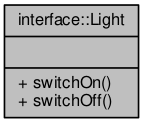
\includegraphics[scale=.5]{img/UML/CollaborationDiagram/interface/interface::Light.png}
	\caption{Collaboration Diagram - interface::Light}
\end{figure}
\begin{figure}[!ht]
	\centering
	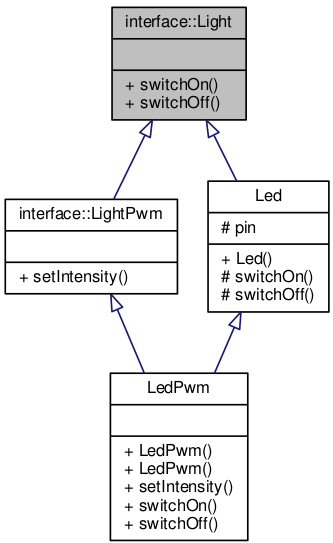
\includegraphics[scale=.35]{img/UML/InheritanceDiagram/interface/interface::Light.png}
	\caption{Inheritance Diagram - interface::Light}
\end{figure}


\subsection{LightPwm.h}
Interfaccia che estende l'interfaccia Light, permettendo di gestire il feedback luminoso dei LED come la variazione dell'intensità luminosa, agendo sui pin PWM.
\subsubsection{Metodi}
\begin{itemize}
	\item \texttt{public virtual void setIntensity(uint8\_t) = 0;}
\end{itemize}
\begin{figure}[!ht]
	\centering
	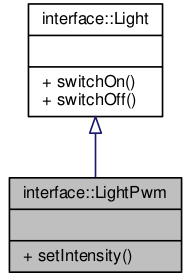
\includegraphics[scale=.45]{img/UML/CollaborationDiagram/interface/interface::LightPwm.png}
	\caption{Collaboration Diagram - interface::LightPwm}
\end{figure}
\begin{figure}[!ht]
	\centering
	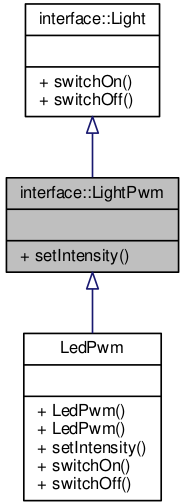
\includegraphics[scale=.35]{img/UML/InheritanceDiagram/interface/interface::LightPwm.png}
	\caption{Inheritance Diagram - interface::LightPwm}
\end{figure}

